
% Nineteen chapter ====================================================
\chapter*{Nineteen}
\addcontentsline{toc}{chapter}{Nineteen}

\begin{flushright}
\parbox{0.8\textwidth}{
\emph{The truth is at the beginning of anything and its end are alike touching. \\
\hspace*{\fill}{\textperiodcentered \textperiodcentered \textperiodcentered \hspace*{0.2em} Yoshida Kenko} } }
\end{flushright}

\noindent
Nineteen is chess variant which is played on 18 x 18 board, with
light gold-yellow and white fields and gold-yellow and dark gray
pieces.In algebraic notation, columns are enumerated from 'a' to 'r',
and rows are enumerated from '1' to '18'. A new piece is introduced,
Star. Star colors are the same as for ordinary pieces, i.e. gold-yellow
and dark gray.

\clearpage % ..........................................................
% Star ****************************************************************

\section*{Star}
\addcontentsline{toc}{section}{Star}

\noindent
\begin{wrapfigure}[11]{l}{0.4\textwidth}
\centering
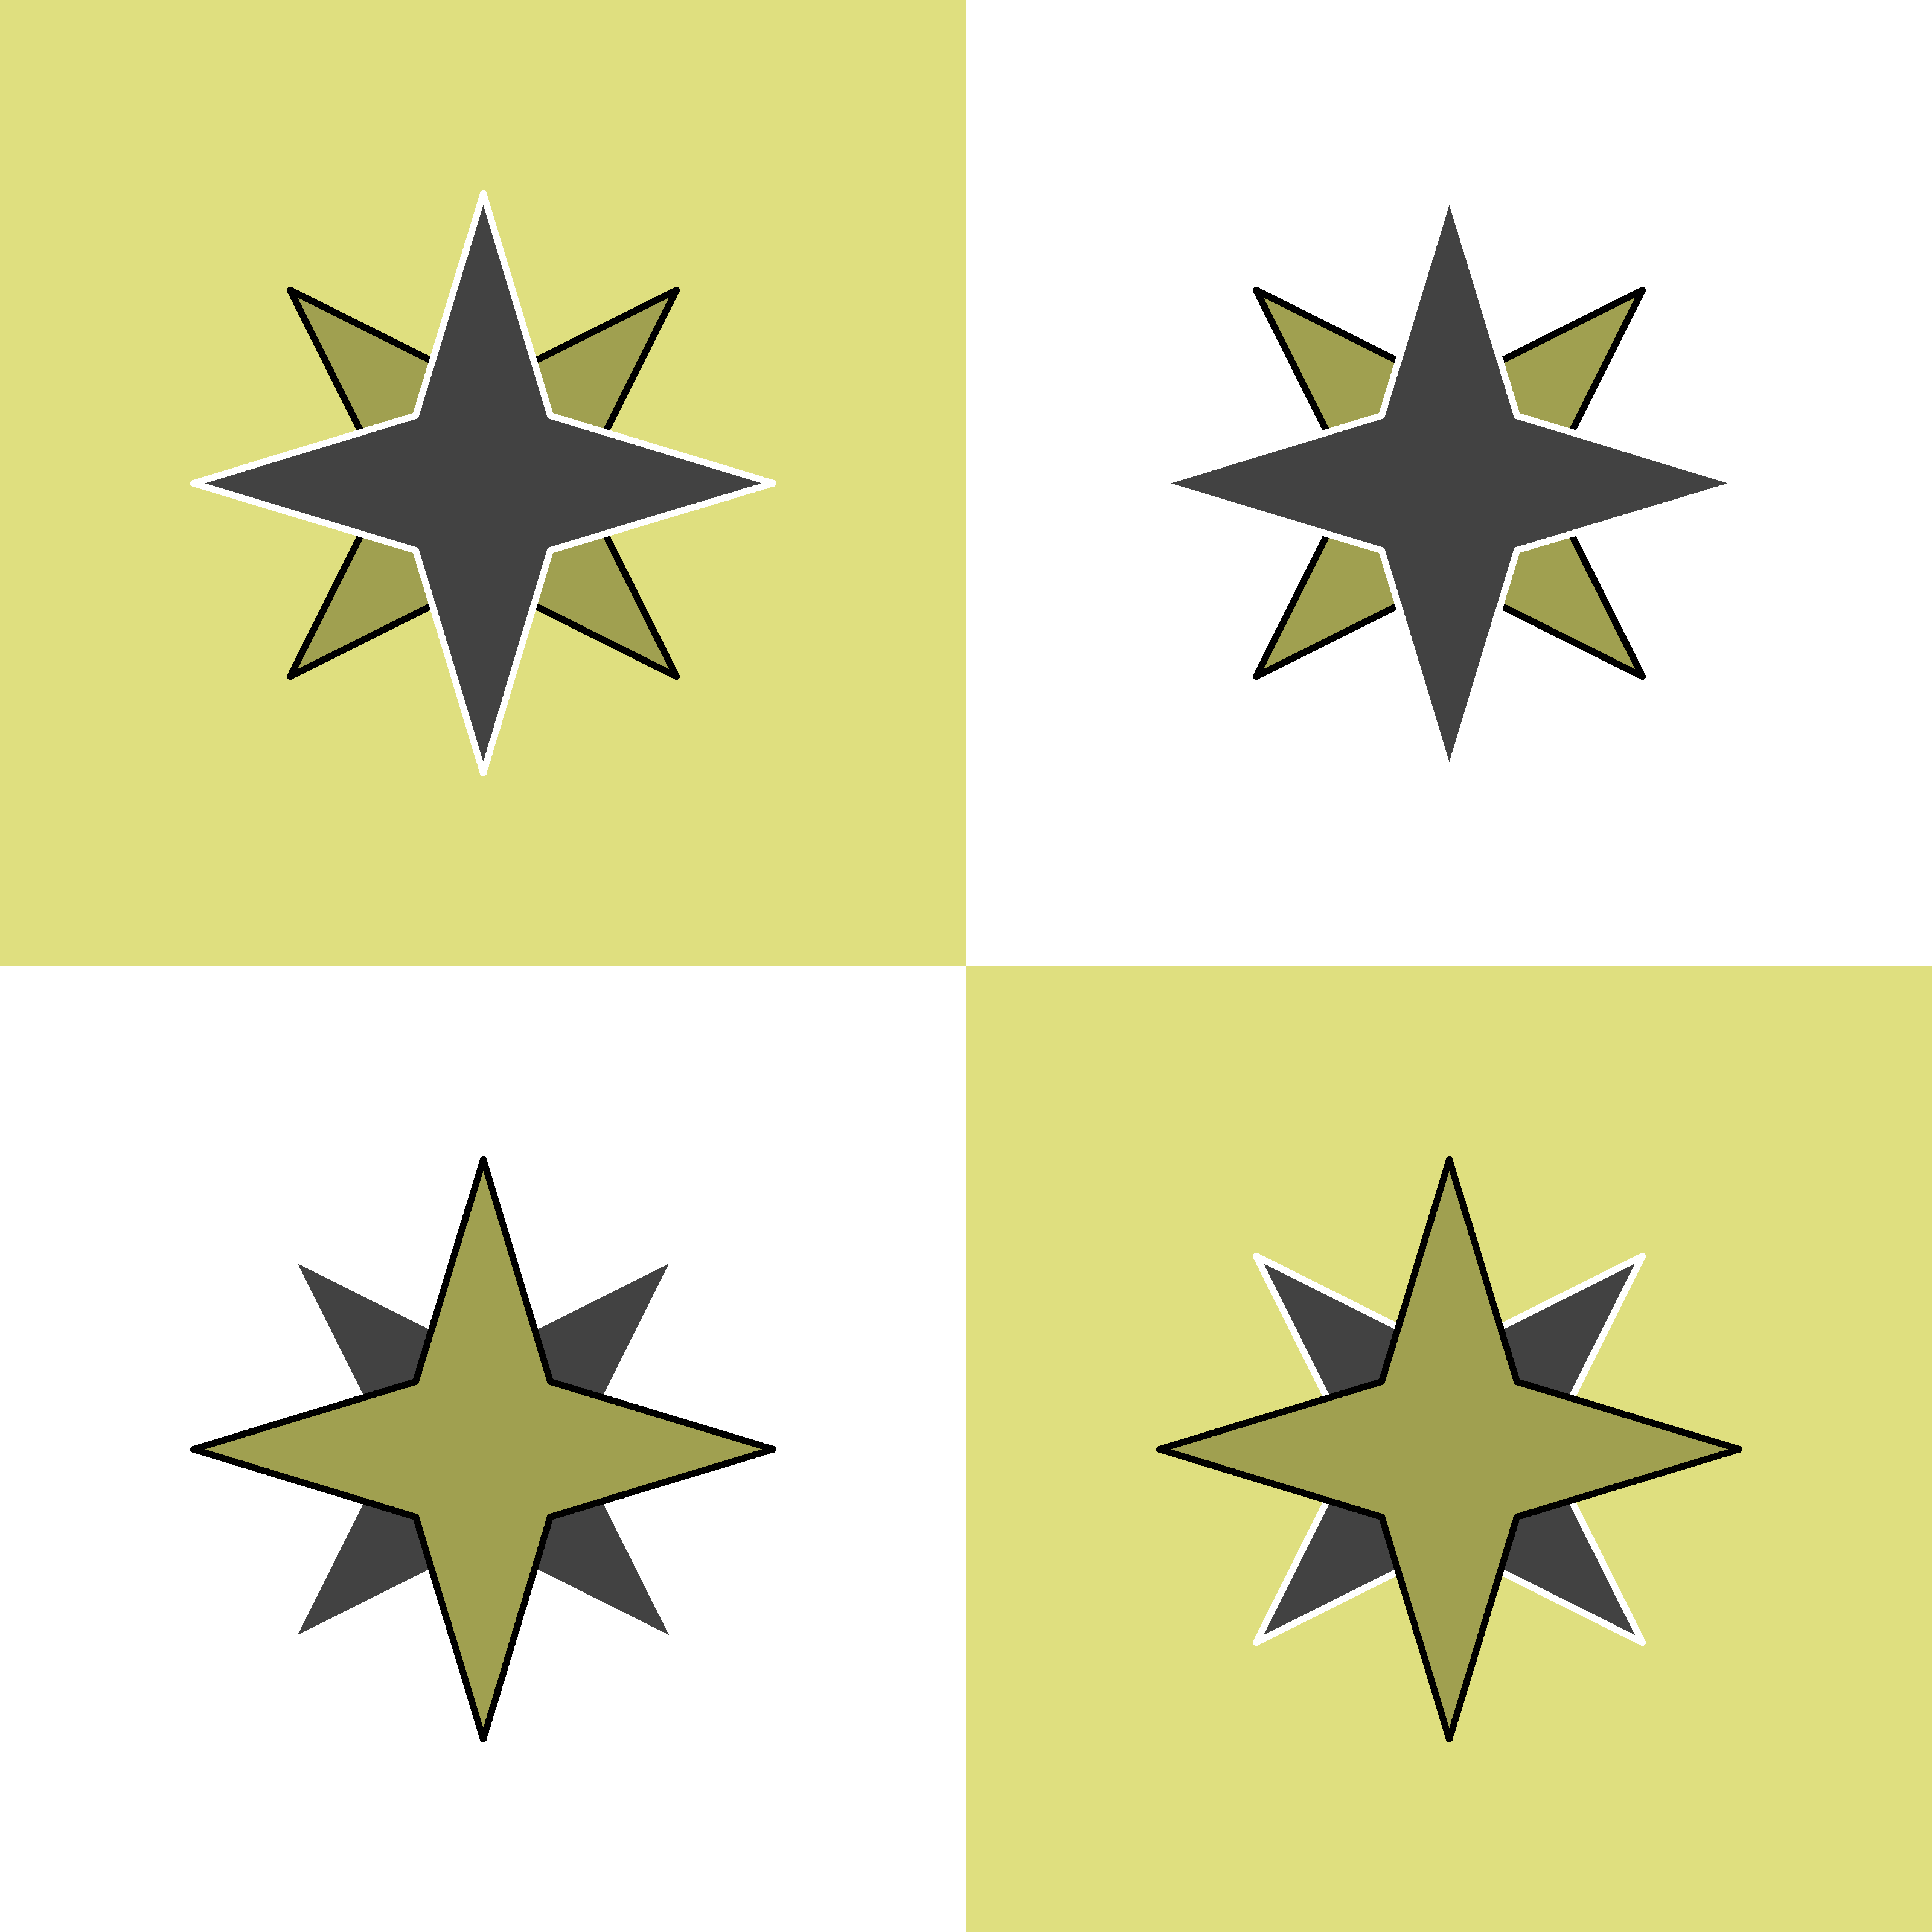
\includegraphics[width=0.4\textwidth, keepaspectratio=true]{pieces/11_star.png}
\caption{Star}
\label{fig:11_star}
\end{wrapfigure}
Star is a dormant piece, it does not belong to any player, and can't be moved by either.

Stars are positioned in very corners of chessboard, light Stars in lower left and upper right
corners, dark Stars in lower right and upper left corners.

Star is a teleporting piece. Teleportation is initiated by any piece diving into a Star, by
touching a Star or field at which it stands (as if trying to capture Star). Piece in question
then reappears on any non-occupied portal-field near Star in opposite color. Any momentum
carried is lost. Teleportation is not limited by matching colors of a piece and a Star, any
piece can use any Star to start teleporting.

Player initiating teleportation can choose which opposite color Star will be destination, and
at which empty portal-field piece will reappear. If there is no empty portal-field near both
opposite color Stars, piece is removed from chessboard as if it has been captured.

Kings cannot be teleported, it's illegal for a King to dive into a Star.

Pawns cannot be promoted to a Star.

In algebraic notation symbol for Star is 'T'.

\clearpage % ..........................................................

\subsection*{Portal-fields}
\addcontentsline{toc}{subsection}{Portal-fields}

\noindent
\begin{wrapfigure}{l}{0.5\textwidth}
\centering
\includegraphics[width=0.388888888889\textwidth, keepaspectratio=true]{examples/12_n/scn_n_01_portal_fields.png}
\caption{Portal-fields}
\label{fig:scn_n_01_portal_fields}
\end{wrapfigure}
Portal-fields are all fields immediately surrounding a particular field
horizontally, vertically and diagonally. They are the same as step-fields
of a King.

Since all Stars are pinned into the corners of a chessboard, there are always
exactly 3 portal-fields around each one.

\subsection*{Teleporting}
\addcontentsline{toc}{subsection}{Teleporting}

All emerging pieces end their teleportation ply on the choosen empty
portal-field. All of momentum carried into teleportation is lost, it cannot
be used neither in the same teleporting move, nor at some point later.
Since this effectively prevents any cascading, teleportation always ends
complete player's move.

\clearpage % ..........................................................

\noindent
\begin{figure}[!h]
% \begin{figure}[!t]
\includegraphics[width=1.0\textwidth, keepaspectratio=true]{examples/12_n/scn_n_02_teleport_init.png}
\caption{Teleportation start}
\label{fig:scn_n_02_teleport_init}
% \centering
\end{figure}

Here, light player is about to dive Wave into upper left dark Star. The only
other option is to dive light Bishop into lower right dark Star, as it is
illegal for King to teleport.

In any case, teleported piece would have to emerge near either light Star.
The only empty portal-field is numbered, so it would have to be upper right
light Star, on field 1.

\clearpage % ..........................................................

\noindent
\begin{figure}[!h]
% \begin{figure}[!t]
\includegraphics[width=1.0\textwidth, keepaspectratio=true]{examples/12_n/scn_n_03_teleport_dark.png}
\caption{Teleporting dark}
\label{fig:scn_n_03_teleport_dark}
% \centering
\end{figure}

After emerging, light Wave lost all of it's momentum, so it's illegal to
e.g. activate light Pyramid after teleportation.

Dark player could dive Rook into dark Star. Since all portal-fields of both
light Stars are now occupied, that would remove dark Rook from chessboard as
if it has been captured.

Only other option is to dive dark Unicorn into light Star.

\clearpage % ..........................................................

\noindent
\begin{figure}[!h]
% \begin{figure}[!t]
\includegraphics[width=1.0\textwidth, keepaspectratio=true]{examples/12_n/scn_n_04_teleport_end.png}
\caption{Teleporting end}
\label{fig:scn_n_04_teleport_end}
% \centering
\end{figure}

With both dark Stars having all of their portal-fields empty, dark Unicorn could
land on any previously numbered portal-field.

% **************************************************************** Star
\clearpage % ..........................................................

\section*{Promotion}
\addcontentsline{toc}{section}{Promotion}

Promotion is non enforced, delayed variety, i.e. it's the same as in
\hyperref[sec:Age of Aquarius/Promotion]{previous chess variant}, Age of Aquarius.

Again, Pawns cannot be promoted to a Star.

Additionaly, promotion in this variant is monogamous.
Only one Queen in the same color can be present on chessboard at any given time.

\clearpage % ..........................................................

\section*{En passant}
\addcontentsline{toc}{section}{En passant}

\noindent
\begin{wrapfigure}{l}{0.4\textwidth}
\centering
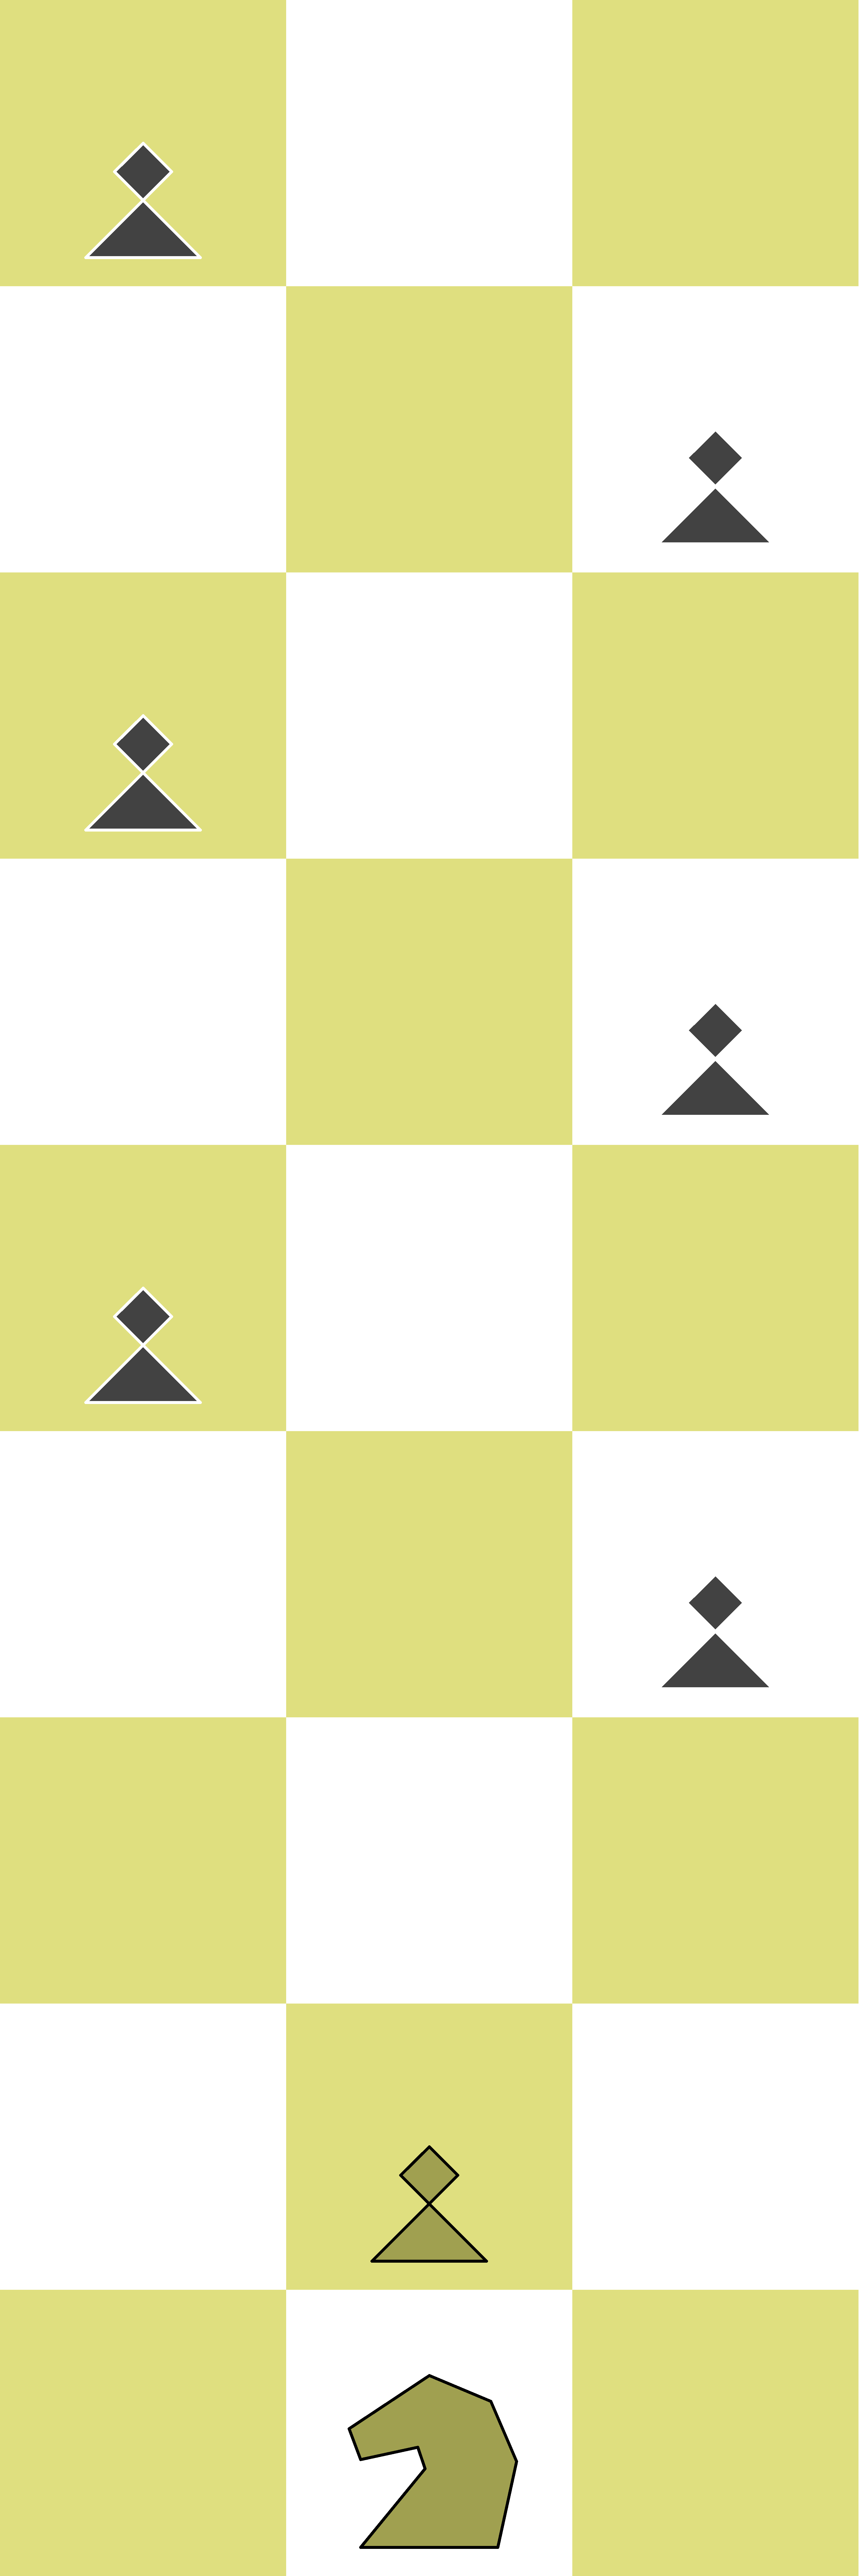
\includegraphics[width=0.166666666667\textwidth, keepaspectratio=true]{en_passants/12_nineteen_en_passant.png}
\caption{En passant}
\label{fig:12_nineteen_en_passant}
\end{wrapfigure}
Rush and en passant are identical to those in Classic Chess, only difference
is that Pawn can now move longer on initial turn, up to 7 fields in this
variant.

\clearpage % ..........................................................

\section*{Castling}
\addcontentsline{toc}{section}{Castling}

Castling is the same as in Classical Chess, only difference is that King can move between 2 and 6 fields across.
All other constraints from Classical Chess still applies.

\noindent
\begin{figure}[!h]
% \begin{figure}[!t]
\includegraphics[width=1.0\textwidth, keepaspectratio=true]{castlings/12_n/nineteen_castling.png}
\caption{Castling}
\label{fig:nineteen_castling}
% \centering
\end{figure}

In example above, all valid King's castling moves are numbered.

\noindent
\begin{figure}[!h]
% \begin{figure}[!t]
\includegraphics[width=1.0\textwidth, keepaspectratio=true]{castlings/12_n/nineteen_castling_left_05.png}
\caption{Castling long left}
\label{fig:nineteen_castling_left_05}
% \centering
\end{figure}

In this example King was castling long to the left. Initial King's position is marked with "K".
After castling is finished, left Rook ends up at field immediately right to the King.

\clearpage % ..........................................................

\section*{Initial setup}
\addcontentsline{toc}{section}{Initial setup}

Stars are positioned in very corners of chessboard, light Stars in lower left and upper right
corners, dark Stars in lower right and upper left corners. Initial setup can be seen in image below:

\noindent
% \begin{figure}[t]
\begin{figure}[h]
\includegraphics[width=1.0\textwidth, keepaspectratio=true]{boards/12_nineteen.png}
\caption{Nineteen board}
\label{fig:12_nineteen}
% \centering
\end{figure}

\clearpage % ..........................................................
% ==================================================== Nineteen chapter
